\section{Phương pháp nghiên cứu}
\subsection{Linear Regression}
Hồi quy tuyến tính là một kỹ thuật thống kê được sử dụng để mô hình hóa mối liên hệ giữa một biến phụ thuộc và một hoặc nhiều biến độc lập. Phương pháp này giả định một mối quan hệ tuyến tính và cố gắng xác định đường thẳng tối ưu nhằm giảm thiểu sự chênh lệch giữa các giá trị dự đoán và quan sát được. Hồi quy tuyến tính được áp dụng để dự đoán kết quả và hiểu về ảnh hưởng của các biến trong các lĩnh vực như kinh tế, tài chính và học máy. Phương pháp này, được giới thiệu bởi nhà thống kê nổi tiếng Sir Francis Galton vào cuối thế kỷ 19, nhằm xác định một phương trình tuyến tính đại diện cho mối quan hệ. Công thức cho hồi quy tuyến tính thường được biểu diễn dưới dạng một phương trình mô tả đường thẳng tối ưu này được biết đến là:
\[y=\beta_0+\beta_1x+\varepsilon\]
Trong đó:\\
	\indent\textbullet\ \(y\) là giá trị dự đoán của biến phụ thuộc (y).\\
	\indent\textbullet\ \(x\) là các biến độc lập.\\
	\indent\textbullet\ \(\beta_0\) là giá trị dự đoán của y khi X bằng 0 (intercept).\\
	\indent\textbullet\ \(\beta_1\) là hệ số hồi quy – cho biết giá trị dự đoán y thay đổi như thế nào khi X thay đổi.\\
	\indent\textbullet\ \(\varepsilon\) là sai số.\\
\\
Công thức tính \(\beta_0\) và \(\beta_1\):\\
\[\beta_1=\frac{\sum\left(x_i-\bar{x}\right)\left(y_i-\bar{y}\right)}{\sum\left(x_i-\bar{x}\right)^2}\]
\[\beta_0=\bar{y}-\beta_1\bar{x}\]
Trong đó:\\
	\indent\textbullet\ \(x_i\) và \(y_i\) là các giá trị cụ thể của biến độc lập và phụ thuộc.\\
	\indent\textbullet\ \(\bar{x}\) và \(\bar{y}\) là giá trị trung bình của \(x\) và \(y\) tương ứng.\\
\\
Công thức tính \(R^2\):
\[R^2=1-\frac{\sum\left(y_i-\hat{y_i}\right)^2}{\sum\left(y_i-\bar{y}\right)^2}\]
Trong đó:\\
	\indent\textbullet\ \(\hat{y_i}\) là giá trị dự đoán của \(y_i\)\\
	\indent\textbullet\ \(\bar{y_i}\) là giá trị trung bình của \(y\)\\

% =========================================
\subsection{ARIMA}
Nội dung.

% =========================================
\subsection{RNN}
Nội dung. 
% =========================================
\subsection{RNN}
\begin{minipage}{0.45\textwidth}
\centering
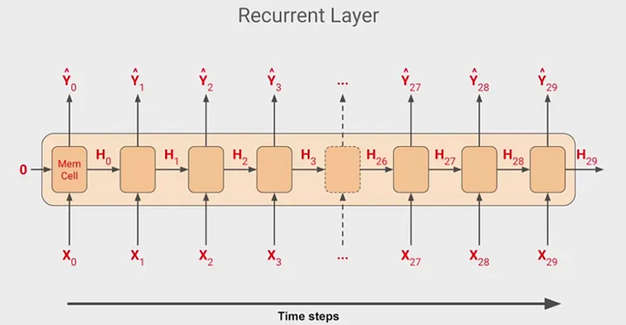
\includegraphics[width=1\textwidth]{resources/chapter-4/rnn-1.png}
\end{minipage}
\[h_t = \sigma (W_{h}x_{t} + U_h h_{t-1} + b_t) \]
\[y_t = \sigma (W_{y} h_t + b_y)\]
    \indent\textbullet\ \(h_t\): Vector lớp ẩn tại thời điểm t\\
    \indent\textbullet\ \(X_t\): vector đầu vào tại thời điểm t\\
    \indent\textbullet\ \(\widehat{Y_t}\): vector đầu ra tại thời điểm t\\
    \indent\textbullet\ \(W_h\), \(U_h\), \(W_y\): Là ma trận trọng số ngẫu nhiên\\
    \indent\textbullet\ \(b_h\), \(b_y\): là các bias\\
    \indent\textbullet\ \(\sigma_h\), \(\sigma_y\): là các hàm kích hoạt\\

Một số hàm kích hoạt phổ biến là:
\\ \textbf{Sigmoid}
\[f(x)=\frac{1}{1+e^{-x}}\]
\\ \textbf{Tanh}
\[f(x) = \frac{e^x - e^{-x}}{e^x + e^{-x}}\]
\\ \textbf{RELU}
\[f(x)=\{\begin{matrix}
0 & \text{for } x<0 \\
x & \text{for } x\ge0
\end{matrix}.\]
Thuật toán
Đầu vào: chuỗi thời gian \(x_1\), \(x_2\), \(x_3\), … \(x_t\), nhãn thực tế tương ứng \(y_1\), \(y_2\), \(y_3\), … \(y_t\),
Đầu ra: Tính toán hàm mất mát (Loss Function) và cập nhật các trọng số \(W_h\), \(U_h\), \(W_y\), \(b_h\), \(b_y\)
\[\text{Loss Function} = \frac{1}{N} \sum_{i=1}^{N} (-y_i + \hat{y_i})^2\]
Lặp lại quá trình trên cho đến khi hàm mất mát giảm đủ ( không thay đổi trong một số bước lặp nhất định, không thể giảm được nữa)
% =========================================
\subsection{LSTM}
Nội dung.

% =========================================
\subsection{GRU}
Nội dung.

% =========================================
\subsection{VARMA}
Nội dung. 

% =========================================
\subsection{Kalman Filter}
Nội dung.

% =========================================
\subsection{Meta-learning}
Nội dung.


% =========================================
\subsection{NBeats}
Nội dung.

% =========================================
\subsection{N-HiTS}
Nội dung.

% =========================================
\subsection{NBeats}
\begin{minipage}{0.45\textwidth}
\centering
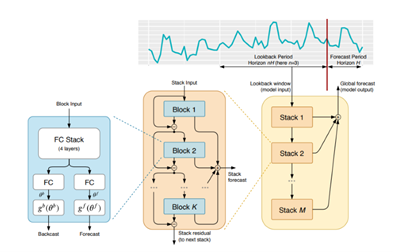
\includegraphics[width=1\textwidth]{resources/chapter-4/nbeats-1.png}
\end{minipage}
\\
\({h}_{\ell,1} = FC_{\ell,1}({x}_{\ell}), \quad {h}_{\ell,2} = FC_{\ell,2}({h}_{\ell,1}), \quad {h}_{\ell,3} = FC_{\ell,3}({h}_{\ell,2}), \quad {h}_{\ell,4} = FC_{\ell,4}({h}_{\ell,3}).\) \\
\(\theta^b_{\ell} = LINEAR_{\ell}^{b}({h}_{\ell,4}), \quad \theta^f_{\ell} = LINEAR_{\ell}^{f}({h}_{\ell,4}).\) \\

\[\widehat{\vec{y}}_{\ell} = \sum_{i=1}^{\dim(\theta^f_{\ell})} \theta^f_{\ell,i} \vec{v}^f_{i}, \quad  \widehat{\vec{x}}_{\ell} = \sum_{i=1}^{\dim(\theta^b_{\ell})} \theta^b_{\ell,i} \vec{v}^b_{i}.
\]
Mô tả cấu trúc mô hình: \\
\\
\textbf{Khối Đầu vào (Time series input)}: của mô hình là một chuỗi thời gian \(Y_{t-n+1:t}\) chứa các đặc điểm của quá khứ.\\
\textbf{Ngăn xếp khối đầu vào (Stack Input)}: cấu trúc này bao gồm các khối được xếp chống lên nhau. Mỗi khối thực hiện 2 nhiệm vụ chính là dự đoán lại quá khư (backcast) và dự báo tương lai(forecast)\\
\textbf{Broadcast}: mỗi khối cố  gắng tại tạo lại đầu vào (phần quá khứ) để dảm phần dư trước khi chuyển trang khối tiếp theo\\
\textbf{Forecast}: Mỗi khi đưa ra dự báo cho tương lai và các dự báo này được tổng hợp lại để tạo ra dự báo cuối cùng\\
\\
\textbf{Fully Connected Layers}: Mỗi khối báo gồm nhiều lớp fully-connected. Các lớp này sử dụng các hàm kích hoạt để học các bieuer diễn phi tuyến của dữ liệu\\
\textbf{Residual Connections(kết nối dư)}: sau mỗi khối, phần dư giữa đầu vào và backcast được tính toán và sử dụng làm đầu vào cho khối tiếp theo\\
\textbf{Global Forcecast}: Dự báo cuối cùng được tạo ra bằng cách tổng hợp các dự báo từ tát cả các khối. Các dự báo này được kết hợp lại để tạo ra dự báo cuối cùng cho chuỗi thời gian tương lai.\\
